\documentclass{article}
\usepackage[utf8]{inputenc}
\usepackage{geometry}
\geometry{left = 15mm, top = 15mm, bottom = 15mm, right = 15mm}
\usepackage{verbatim}
\usepackage{graphicx}
\usepackage{wrapfig}
\usepackage{amsmath}
\usepackage{fullpage}
\usepackage{hyperref}
\usepackage{graphicx}
\usepackage{listings}
\usepackage{color}

\definecolor{mygreen}{rgb}{0,0.6,0}
\definecolor{mygray}{rgb}{0.5,0.5,0.5}
\definecolor{mymauve}{rgb}{0.58,0,0.82}

\lstset{ 
  backgroundcolor=\color{white},   % choose the background color; you must add \usepackage{color} or \usepackage{xcolor}; should come as last argument
  basicstyle=\footnotesize,        % the size of the fonts that are used for the code
  breakatwhitespace=false,         % sets if automatic breaks should only happen at whitespace
  breaklines=true,                 % sets automatic line breaking
  captionpos=b,                    % sets the caption-position to bottom
  commentstyle=\color{mygreen},    % comment style
  deletekeywords={...},            % if you want to delete keywords from the given language
  escapeinside={\%*}{*)},          % if you want to add LaTeX within your code
  extendedchars=true,              % lets you use non-ASCII characters; for 8-bits encodings only, does not work with UTF-8
  firstnumber=1,                   % start line enumeration with line 1000
  frame=single,	                   % adds a frame around the code
  keepspaces=true,                 % keeps spaces in text, useful for keeping indentation of code (possibly needs columns=flexible)
  keywordstyle=\color{blue},       % keyword style
  language=Python,                 % the language of the code
  morekeywords={*,...},            % if you want to add more keywords to the set
  numbers=left,                    % where to put the line-numbers; possible values are (none, left, right)
  numbersep=5pt,                   % how far the line-numbers are from the code
  numberstyle=\tiny\color{mygray}, % the style that is used for the line-numbers
  rulecolor=\color{black},         % if not set, the frame-color may be changed on line-breaks within not-black text (e.g. comments (green here))
  showspaces=false,                % show spaces everywhere adding particular underscores; it overrides 'showstringspaces'
  showstringspaces=false,          % underline spaces within strings only
  showtabs=false,                  % show tabs within strings adding particular underscores
  stepnumber=1,                    % the step between two line-numbers. If it's 1, each line will be numbered
  stringstyle=\color{mymauve},     % string literal style
  tabsize=4,	                   % sets default tabsize to 2 spaces
  title=\lstname                   % show the filename of files included with \lstinputlisting; also try caption instead of title
}


\title{Numerical Recipes for Astrophysics \\ Second hand-in homework exercise}
\author{Zorry Belcheva}
\date{May 2019}

\begin{document}

\maketitle

\section{Exercise 1: Normally distributed pseudo-random numbers}

\subsection{Part a: RNG}
The aim of this exercise is to create and test a random number generator (RNG) that is a combination of a Multiply-with-carry RNG and a 64-bit XOR-shift algorithm. First, the script reads the seed from a file \verb+seed.txt+, taking the global seed value to be the last in the list. For the first run of this exercise, the seed is set to 3310934475, subsequent runs of the other scripts append to this file. The \verb+lcg_float()+ function returns a pseudorandom number between 0 and 1 generated using the seed using a linear congruential RNG (or any number less than the chosen modulus, if used with \verb+float=False+). The constants used for the LCG are those of the Borland C/C++ implementations. A couple of other options were tested, and these produced best results. Other options are also discussed in the comments of the code. The function \verb+xorshift()+ can be used to shift the bits of the seed in a certain sequence to produce another random number (which is a 64-bit integer and is not between 0 and 1). In order  to do this without letting Python influence the data type, the bit shift parameters \verb+a1+, \verb+a2+ and \verb+a3+ are also cast to type \verb+np.int64()+. The implementation in this code uses values for these parameters that ensure all 64 bits of the seed are shuffled (and not just the first 32), and the chain has a period of $2^{64}-1$. \footnote{Credit for the values: Wikipedia - Xorshift/Example implementation.} The \verb+create_random()+ function generates random numbers by first using \verb+xorshift()+ with the current (global) seed, and then calls \verb+lcg_float()+ which in turn uses the new XOR-shifted global seed as a base to create a random number between 0 and 1, and returns it. The \verb+create_random()+ function can generate an array of random numbers of size = \verb+size+ provided by the user. 

Additionally, the functions \verb+avg()+ and \verb+standard_dev()+ are implemented to calculate, respectively, the average and standard deviation of a sample \verb+x+.

Tests were carried on the RNG:
\begin{itemize}
    \item Plotting 1000 sequential random numbers against each other in a scatter plot, i.e. $x_{i+1}$ vs. $x_i$.
    \item Plotting the value of the first 1000 random numbers vs. their index from 0 to 999.
    \item Plotting a histogram of the first 1 000 000 random numbers binned in 20 bins of width 0,05.
    \item Examining the scatter around the mean number count in the 20 bins containing 1 000 000 numbers.
\end{itemize}

The code that runs these tests is given by:
\lstinputlisting[language=Python, firstline=1]{ex1a.py}

The output of the code is just the updated global seed value, and print statements used to verify the tests were carried out. Also for the 4th additional test, the standard deviation and average of the counts in the 20 bins are printed out in order to examine whether the RNG produces a reasonable scatter around the expected mean of 1 000 000 / 20 = 50 000 numbers per bin. The latest seed value is appended to the file \verb+seed.txt+ for the next script to use. 

\lstinputlisting{./output/ex1a.txt}

As seen from the output, the standard deviation of the scatter around the mean of number counts is 202.4 and the mean itself is 50000.0. The standard deviation should in principle not be more than $\sqrt{N} = \sqrt{50000} \simeq 223.6$. Our RNG falls within this bound, and all bin counts are within 2 standard deviations $2\sigma$ from the mean (see figure \ref{fig:RNGtest3_zoom}), meaning the RNG performs well enough. 

The code has made three plots in the \verb+plots+ directory for the three tests: figure \ref{fig:RNGtest1} shows the first 1000 numbers against each other, figure \ref{fig:RNGtest2} shows their value against their index, and figure \ref{fig:RNGtest3} shows the uniformity of the RNG. As seen from the three plots, the RNG produces numbers that do appear to be (pseudo)random and not predictable, and their distribution is quite uniform. The fourth plot showing a zoom-in of the scatter in the bin counts puts into perspective the way the bin counts vary. As discussed in the previous paragraph, given all bin counts are within $2\sigma$ of the average, the RNG can be taken as good for our purposes in this assignment.

\begin{figure}[!h]
\centering
\begin{minipage}[t]{8cm}
	\centering
	\includegraphics[width=8cm]{./plots/RNGtest1.pdf}
	\caption{1000 random numbers against each other.}
	\label{fig:RNGtest1}
\end{minipage}%
\quad
\begin{minipage}[t]{8cm}
    \centering
	\includegraphics[width=8cm]{./plots/RNGtest2.pdf}
	\caption{Value of the first 1000 random numbers vs. their index.}
	\label{fig:RNGtest2}
\end{minipage}%
\end{figure}

\begin{figure}[!h]
\centering
\begin{minipage}[t]{8cm}
    \centering
	\includegraphics[width=8cm]{./plots/RNGtest3.pdf}
	\caption{Histogram of the first 1 000 000 random numbers generated, binned in 20 bins of width 0,05.}
	\label{fig:RNGtest3}
\end{minipage}%
\quad
\begin{minipage}[t]{8cm}
    \centering
	\includegraphics[width=8cm]{./plots/RNGtest3_zoomin.pdf}
	\caption{Zoom of the histogram of the first 1 000 000 random numbers generated, showing 2 sigma regions of the scatter around the mean bin count.}
	\label{fig:RNGtest3_zoom}
\end{minipage}%
\end{figure}

\subsection{Part b: Box-Muller transform}
After implementing an RNG that outputs uniformly distributed numbers between 0 and 1, we can use the Box-Muller transform method to generate normally-distributed random numbers. The Box-Muller transforms are as follows: if the numbers $z_1$ and $z_2$ are independent random numbers drawn from a uniform distribution, then $r_1$ and $r_2$, given by
\begin{equation}
    r_1 = \cos{2\pi z_2}\sqrt{-2\log{z_1}} \quad \text{and}  \quad
    r_2 = \sin{2\pi z_2}\sqrt{-2\log{z_1}},
\end{equation}
are independent random numbers drawn from a standard normal distribution, that is a Gaussian with mean 0 and standard deviation 1. In the \verb+ex1b.py+ script, the \verb+create_random_normal_2d()+ function creates normally distributed random numbers by applying the Box-Muller transforms. It gets $z_1$ and $z_2$ by calling the \verb+create_random()+ function, discussed in the previous subsection. The \verb+two_dim+ parameter can be set to \verb+True+ for the function to output a 2D set of random numbers; it is by default set to \verb+False+. The numbers can then be shifted to a Gaussian distribution with different mean $\mu$ and standard deviation $\sigma$ by the \verb+mapping()+ function. It works by first multiplying the numbers by $\sigma$, and then adding $\mu$. In order to test the distribution of the random numbers, the script performs the following tests: creates (2 sets of, just for comparison purposes) 1000 normally-distributed random numbers, and uses the \verb+mapping()+ function to map them to $\mu = 3$ and $\sigma=2.4$. The mapped numbers are then plotted in a normalised histogram, i.e. with each bin scaled by dividing by the sample size. For comparison, a Gaussian $G(\mu=3, \sigma=2.4)$ is overplotted. Additionally, another representation of the 2D random normal numbers is made by plotting them against each other, i.e. each point is a pair generated by \verb+create_random_normal_2d()+. If the distribution is normal, they should be scattered to fill a circle, more concentrated near the origin. 

The functions described are given by the following code (functions from 1a: \verb+lcg_float()+, \verb+xorshift()+, \verb+create_random()+ are omitted for clarity):
\lstinputlisting[language=Python, firstline=56]{ex1b.py}

The code output is again the seed values and print statements to track the progress of the code:
\lstinputlisting{./output/ex1b.txt}

The code has produced 2 figures: figure \ref{fig:BM} contains the normalised histogram (to integrate to 1, i.e. all bins have been divided by the total number of points $n=1000$) of the first 2 sets (one of which could be omitted, this is just to show not all sets would produce equivalent histograms) of 1000 normal random numbers drawn from $Gaussian(\mu=3, \sigma=2.4)$ with a true Gaussian PDF overplotted in black, the mean and regions indicating $1\sigma$, $2\sigma$, $3\sigma$, $4\sigma$ and $5\sigma$ are shown with dashed lines. Figure \ref{fig:G2D} shows a scatter plot of the 1000 random number pairs (standard normal, not mapped to different mean and standard deviation). As seen from the figures, the generated numbers follow the expected Gaussian distribution well. 

\begin{figure}
	\centering
	\includegraphics[width=10cm]{./plots/box-muller.pdf}
	\caption{Normalised histogram of 2 sets of normally distributed random numbers drawn from $G(\mu=3, \sigma=2.4)$ generated with the functions described in section 1.2, with bin counts divided by the sample size such that the y axis now represents a probability density function (PDF). For comparison, the corresponding true Gaussian PDF is shown in black. The modified mean is shown in grey, and coloured dashed lines indicate the $1\sigma$, $2\sigma$, $3\sigma$, $4\sigma$ and $5\sigma$ regions.}
	\label{fig:BM}
\end{figure}

\begin{figure}
	\centering
	\includegraphics[width=9.cm]{./plots/normal-rands-2d.pdf}
	\caption{Scatter plot of 1000 normally-distributed random number pairs, drawn from $G(\mu=0, \sigma=1)$. If truly normal, the randoms should scatter in a circular manner, more concentrated around the origin (red cross).}
	\label{fig:G2D}
\end{figure}

\subsection{Part c: Kolmogorov-Smirnov test}
The Kolmogorov-Smirnov (KS) test can be used to test whether a given sample is consistent with another sample or distribution. The test statistic is the maximum difference $D$ between the two cumulative distribution functions (CDF) of the sample and function in comparison. A p-value can then be estimated using this statistic.

The implementation of the KS-test and using it to test whether \verb+create_random_normal_2d()+ produces normally distributed numbers is given by the following code, again omitting the functions repeated by previous parts:
\lstinputlisting[language=Python, firstline=78]{ex1c.py}

The main part of the function draws a sample of $10^5$ random numbers using \verb+create_random_normal_2d()+, and then using a loop performs the KS test, starting from the first 10 numbers from the drawn sample, and increasing the sample size until all $10^5$ have been tested, using a spacing of 0.1 dex. For comparison, the \verb+scipy+ test is also carried out. The implemented KS test uses different ways to calculate numerically the p-value, using the equations on page 334 of \textit{Numerical Recipes}, based on conditions on the value of $z = D\times (\sqrt{N} + 0.12 + 0.11/\sqrt{N})$. To test whether the sample follows a normal distribution, we need its CDF. For this, the \verb+cdf_gaussian()+ (lines 56-59) function is used. It is an implementation of the definition of the CDF of a Gaussian, and uses the error function, which is in turn implemented as \verb+error_func()+ (lines 48-53), and calculates using numerical integration with the simple trapezium rule implemented in \verb+trapezium()+ (lines 34-45). For the comparison with the \verb+scipy+ implementation, the argument \verb+'norm'+ is used. 

The code output is, again, print statements regarding progress of the code, the time elapsed (to check as this is a heavy part of this homework), and seed values:

\lstinputlisting{./output/ex1c.txt}

The code has produced a plot, figure \ref{fig:KS} that shows both the $D$ statistic of the KS-test and the probability that the sample is drawn from a normal distribution (which is 1 minus the p-value) as a function of the size of the drawn sample. Both axis are logarithmic. Two- and three-sigma confidence regions are also shown in the probability part of the plot. If the probability falls below the 2$\sigma$ line, we can interpret this as `it is unlikely that the sample was drawn from a normal distribution'. Here we see that there are some fluctuations, but overall both the $D$ statistic and the probability are in good agreement with the \verb+scipy+ values, and both could be used to confirm the null hypothesis, which is that this sample was drawn from a normal distribution.

\begin{figure}
	\centering
	\includegraphics[width=11cm]{./plots/KStest.pdf}
	\caption{\textbf{Lower}: KS-test statistic D as a function of size of the drawn sample. The lower the value, the more likely it is that we are using the test to compare the sample with the correct distribution. The scipy implementation is shown with grey crosses for comparison. Axes are logarithmic. \textbf{Upper}: probability that the sample was drawn from a normal distribution, i.e. 1 - p-value given by the KS test, both for this implementation and from scipy. Axes are logarithmic. If the value falls below the 2 sigma line, the null hypothesis is very unlikely.}
	\label{fig:KS}
\end{figure}

\subsection{Pard d: Kuiper test}
The Kuiper test is a generalisation of the KS test that uses as statistic the sum of the most positive and most negative difference between the two CDFs being compared: $V = D_{-} + D_{+}$. 

The implementation of the Kuiper test and using it to test whether \verb+create_random_normal_2d()+ produces normally distributed numbers is given by the following code, omitting modules repeated by previous parts:
\lstinputlisting[language=Python, firstline=78]{ex1d.py}

The code is similar to the one used for the KS-test. The \verb+kuiper_test()+ function returns the value of the $V$ statistic and the probability that the sample is drawn from the inferred distribution with CDF = \verb+cdf+ given in the arguments. The values used to calculate \verb+Q_kuiper+ are found in the book \textit{Numerical Recipes} again. In the main part of the script, values given by \verb+astropy+ are also calculated for comparison. Both the \verb+astropy+ version and the here implemented Kuiper test use the function \verb+cdf_gaussian()+ to calculate the CDF of the normal distribution. Samples are drawn same as in exercise 1c. The Kuiper test, being a generalisation of the KS-test, is likely to produce more reliable results, however both tests are much more sensitive near the median of the distribution and not near its tails, and the user should be aware of this. 

The code output is, again, print statements regarding progress of the code, the time elapsed (to check again, as this is a heavy part of this homework), and seed values:
\lstinputlisting{./output/ex1d.txt}

The code has produced a plot, figure \ref{fig:Kuiper}, very similar to the one in exercise 1c. This implementation is in good agreement with the results obtained from \verb+astropy+, except at the end near $10^5$ points, where \verb+astropy+ wants to reject the null hypothesis, and this implementation still keeps the probability high, which is good, given that we know the null hypothesis i.e. `the random numbers were drawn from a normal distribution' is, in fact, true (of course, relying on the \verb+create_random_normal_2d()+ function). 

\begin{figure}
	\centering
	\includegraphics[width=11cm]{./plots/Kuipertest.pdf}
	\caption{\textbf{Lower}: Kuiper test statistic V as a function of size of the drawn sample. The lower the value, the more likely it is that we are using the test to compare the sample with the correct distribution. The astropy implementation is shown with grey crosses for comparison. Axes are logarithmic. \textbf{Upper}: probability that the sample was drawn from a normal distribution, given by the Kuiper test, both for this implementation and from astropy. Axes are logarithmic. If the value falls below the 2 sigma line, the null hypothesis is very unlikely.}
	\label{fig:Kuiper}
\end{figure}

\subsection{Part e: testing datasets}
\subsubsection{Implementation and code output/results}
10 datasets are examined in this part. The KS test is used to test if any set is consistent with Gaussian pseudo random numbers drawn from $G(\mu=0, \sigma=1)$. For this we don't use directly the CDF of the Gaussian distribution as in parts c and d, but instead use random numbers generated by the implemented standard normal RNG \verb+create_random_normal_2d()+.  To calculate the CDF of our random numbers, the function \verb+get_cdf_value+ takes the sample and the number x, and counts how many points of the sample are less than x. The fraction is then returned. This way $cdf(x_{min})=0$, and $cdf(x_{max})=1$. 

The code that imports the .txt file, performs the KS test on the 10 data sets, and saves the resulting plots is given by:
\lstinputlisting[language=Python, firstline=114]{ex1e.py}

The output of the code is the seed values and the time elapsed:
\lstinputlisting{./output/ex1e.txt}

The code has produced 10 plots, figures \ref{fig:KS-1} to \ref{fig:KS-10}, one for each data set. Each plot contains 3 panels, top and middle are equivalent as those for the KS-test (figure \ref{fig:KS}), except now there is no reference. An additional bottom panel is added to show a histogram of the examined data set.

\subsubsection{Interpretation of results}
Based on the 10 plots produced, given the null hypothesis `this set was drawn from a Gaussian distribution with mean 0 and $\sigma = 1$', we can say that:
\begin{itemize}
    \item Set 1: histogram doesn't match so good, and the probability rejects the hypothesis.
    \item Set 2: obviously not Gaussian when histogram is shown, the probability absolutely rejects the hypothesis also.
    \item Set 3: looks similar to the desired Gaussian, but the probability can be used to claim that likely it isn't, as it's close to the 2 sigma border in the end and fluctuates a lot.
    \item Set 4: looks similar to a the desired Gaussian, but given the behaviour of the probability, likely isn't.
    \item Set 5: both probability and histogram reject hypothesis, KS statistic as well.
    \item Set 6: according to p-value, highly likely it is drawn from the same distribution, however histogram doesn't look so convincing. Maybe this is due to the KS test being more sensitive around the median.
    \item Set 7: p-value behaviour is good, KS statistic very low in the end, histogram confirming as well that most likely this is drawn from the correct distribution.
    \item Set 8: Although the p-value fluctuates, in the end both it and the KS statistic `confirm' the hypothesis. Histogram also seems somewhat convincing that this is the correct Gaussian.
    \item Set 9: the p-value, the KS statistic and the histogram obviously reject the null hypothesis here.
    \item Set 10: The probability drops to less than 3 sigma in the end, KS statistic stays high, histogram confirms this most likely isn't drawn from the desired Gaussian.
\end{itemize}

\begin{figure}[!h]
\centering
\begin{minipage}[t]{7.6cm}
    \centering
    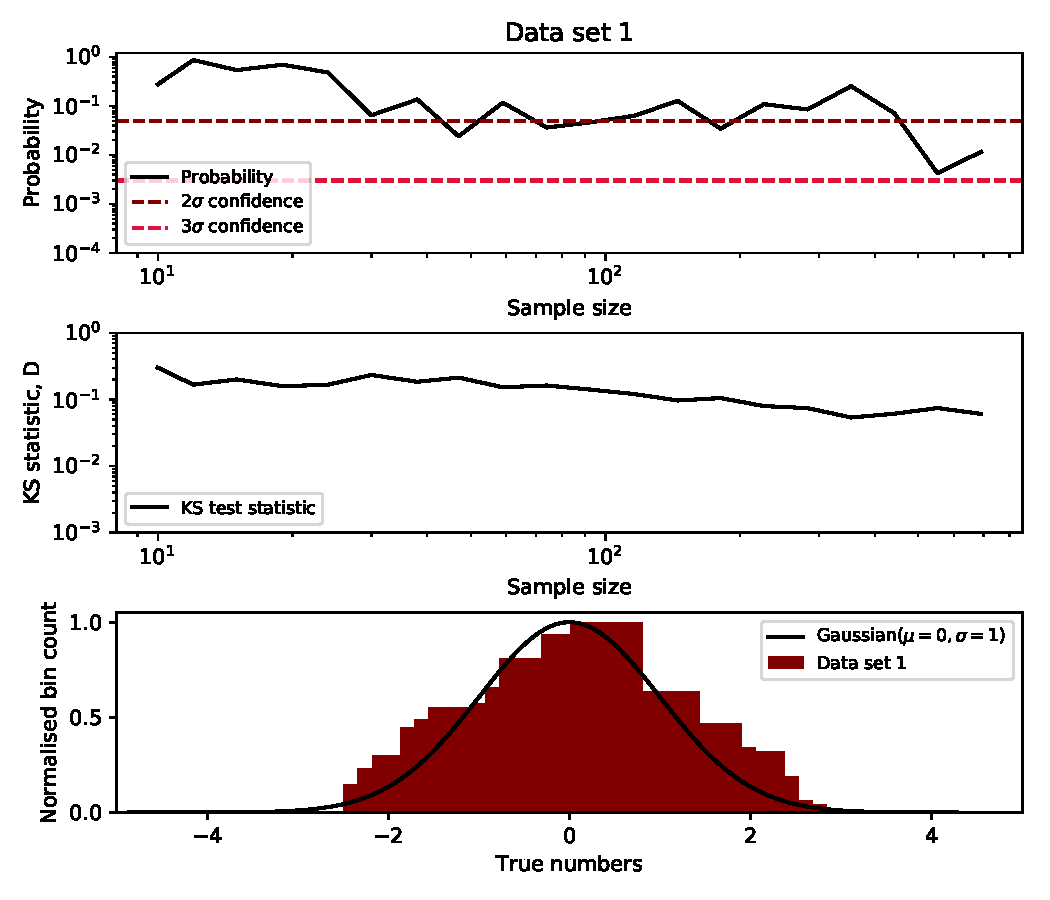
\includegraphics[width = 7.6cm]{./plots/KStest-set1.pdf}
    \caption{\textbf{Upper}: Probability that set 1 matches with a random normal sample; \textbf{middle}: KS-test statistic value; \textbf{lower}: histogram of data set with overlaid Gaussian.}
    \label{fig:KS-1}
\end{minipage}%
\qquad
\begin{minipage}[t]{7.6cm}
    \centering
    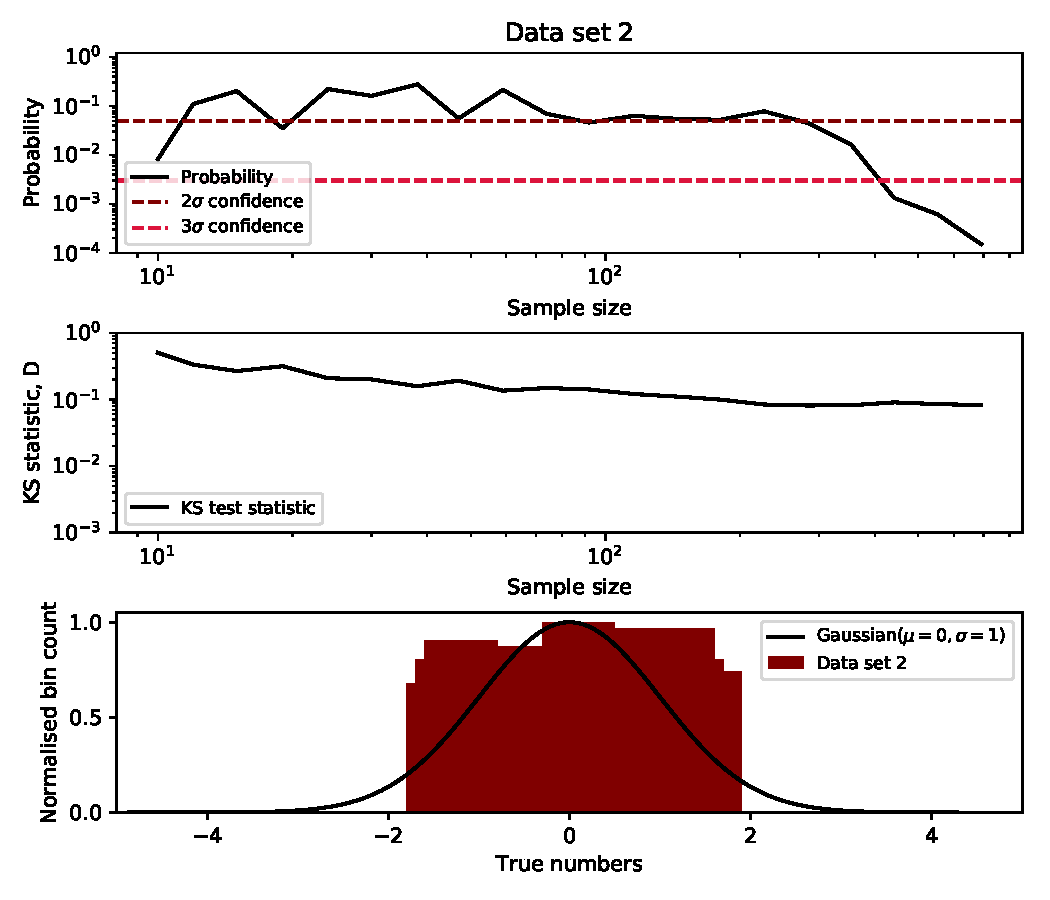
\includegraphics[width = 7.6cm]{./plots/KStest-set2.pdf}
    \caption{\textbf{Upper}: Probability that set 2 matches with a random normal sample; \textbf{middle}: KS-test statistic value; \textbf{lower}: histogram of data set with overlaid Gaussian.}
    \label{fig:KS-2}
\end{minipage}%
\end{figure}

\begin{figure}[!h]
\centering
\begin{minipage}[t]{7.6cm}
    \centering
    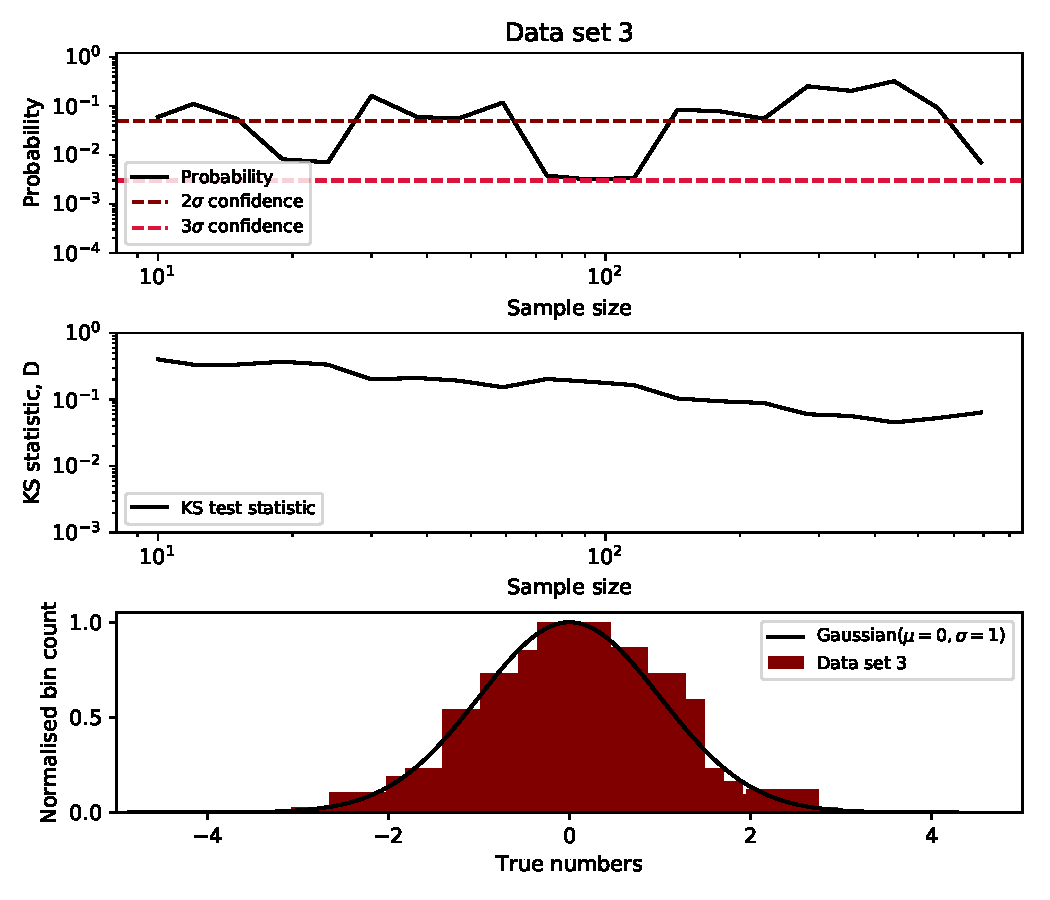
\includegraphics[width = 7.6cm]{./plots/KStest-set3.pdf}
    \caption{\textbf{Upper}: Probability that set 3 matches with a random normal sample; \textbf{middle}: KS-test statistic value; \textbf{lower}: histogram of data set with overlaid Gaussian.}
    \label{fig:KS-3}
\end{minipage}%
\qquad
\begin{minipage}[t]{7.6cm}
    \centering
    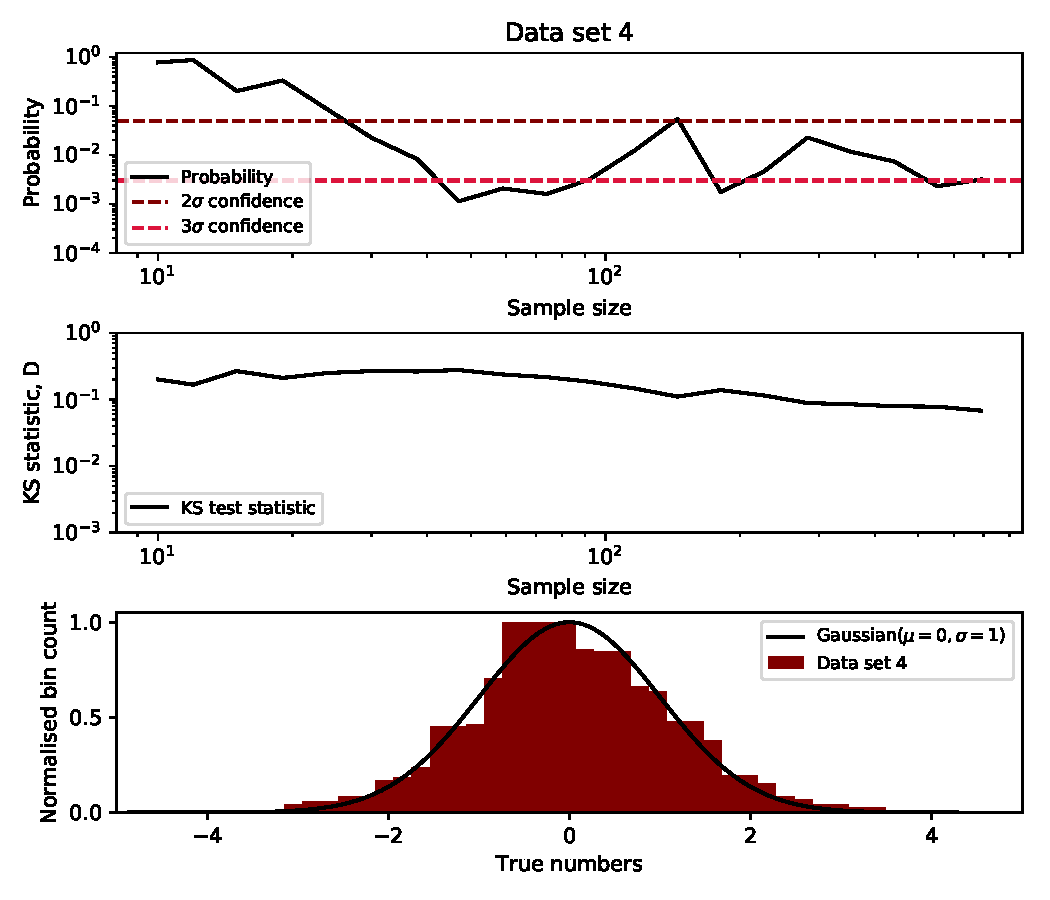
\includegraphics[width = 7.6cm]{./plots/KStest-set4.pdf}
    \caption{\textbf{Upper}: Probability that set 4 matches with a random normal sample; \textbf{middle}: KS-test statistic value; \textbf{lower}: histogram of data set with overlaid Gaussian.}
    \label{fig:KS-4}
\end{minipage}%
\end{figure}

\begin{figure}[!h]
\centering
\begin{minipage}[t]{7.6cm}
    \centering
    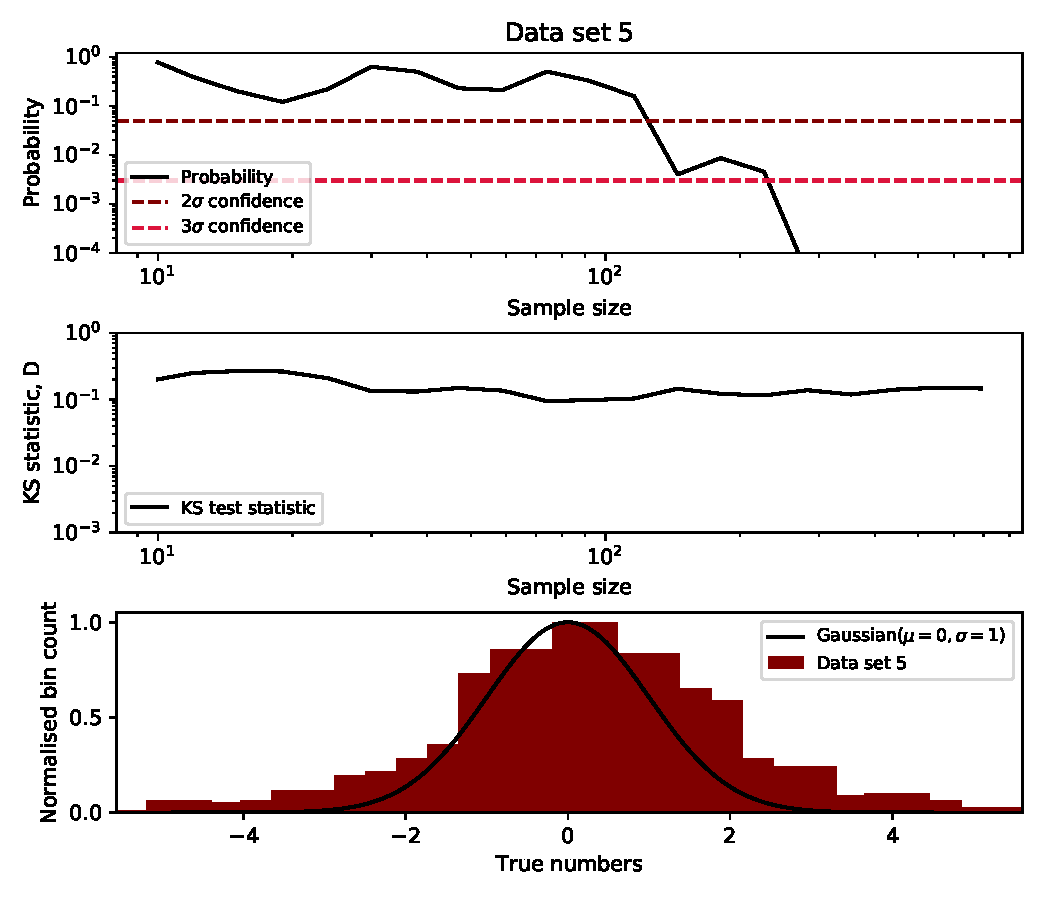
\includegraphics[width = 7.6cm]{./plots/KStest-set5.pdf}
    \caption{\textbf{Upper}: Probability that set 5 matches with a random normal sample; \textbf{middle}: KS-test statistic value; \textbf{lower}: histogram of data set with overlaid Gaussian.}
    \label{fig:KS-5}
\end{minipage}%
\qquad
\begin{minipage}[t]{7.6cm}
    \centering
    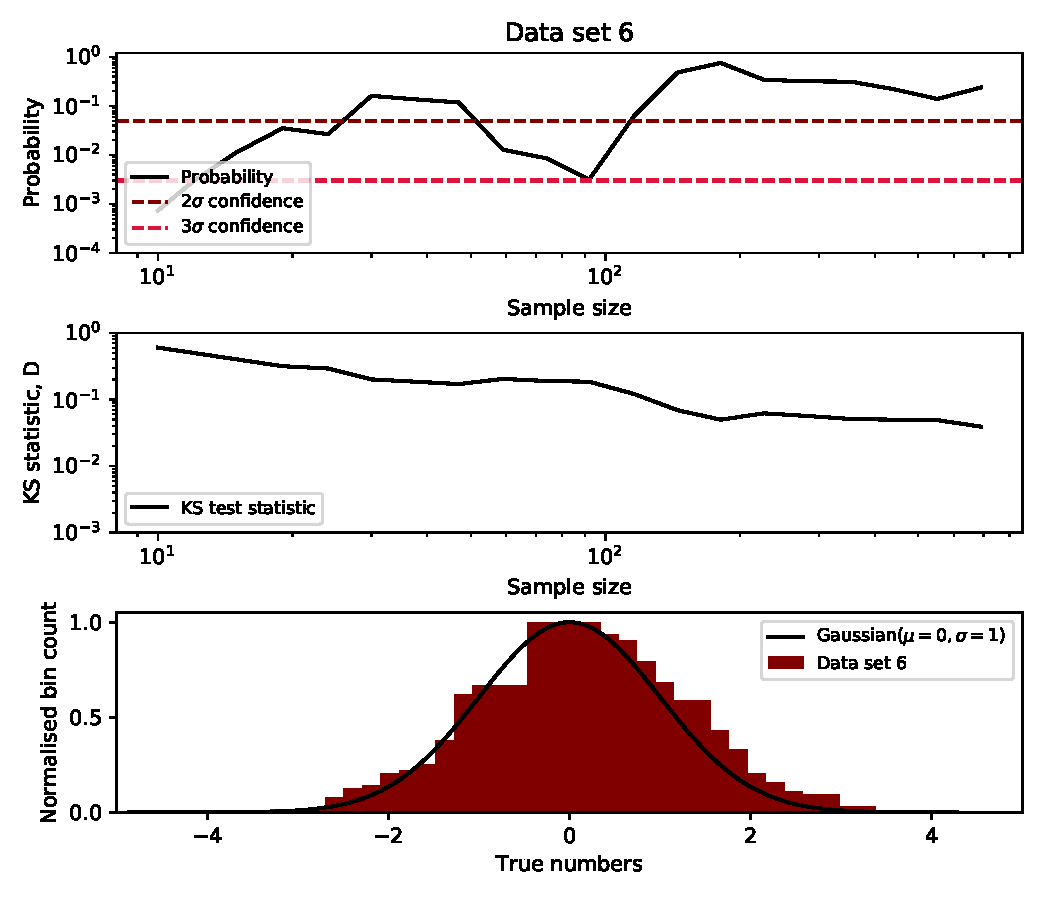
\includegraphics[width = 7.6cm]{./plots/KStest-set6.pdf}
    \caption{\textbf{Upper}: Probability that set 6 matches with a random normal sample; \textbf{middle}: KS-test statistic value; \textbf{lower}: histogram of data set with overlaid Gaussian.}
    \label{fig:KS-6}
\end{minipage}%
\end{figure}

\begin{figure}[!h]
\centering
\begin{minipage}[t]{7.6cm}
    \centering
    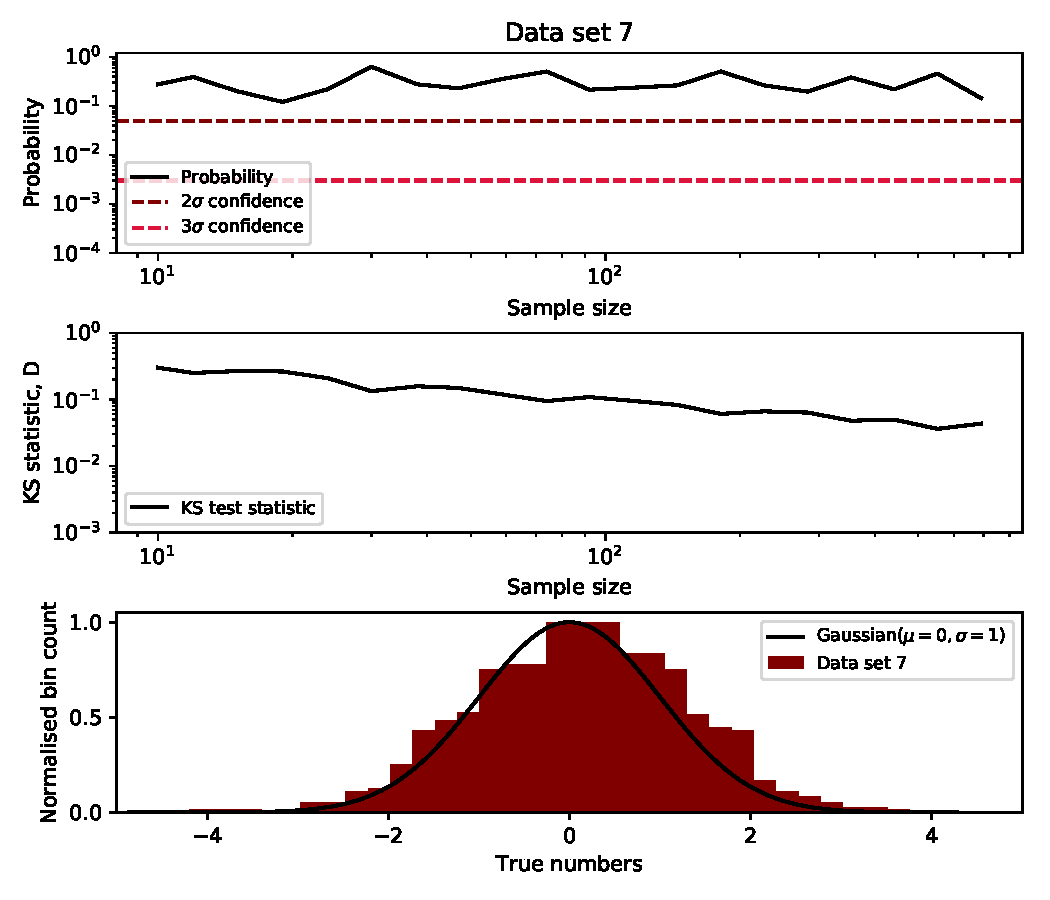
\includegraphics[width = 7.6cm]{./plots/KStest-set7.pdf}
    \caption{\textbf{Upper}: Probability that set 7 matches with a random normal sample; \textbf{middle}: KS-test statistic value; \textbf{lower}: histogram of data set with overlaid Gaussian.}
    \label{fig:KS-7}
\end{minipage}%
\qquad
\begin{minipage}[t]{7.6cm}
    \centering
    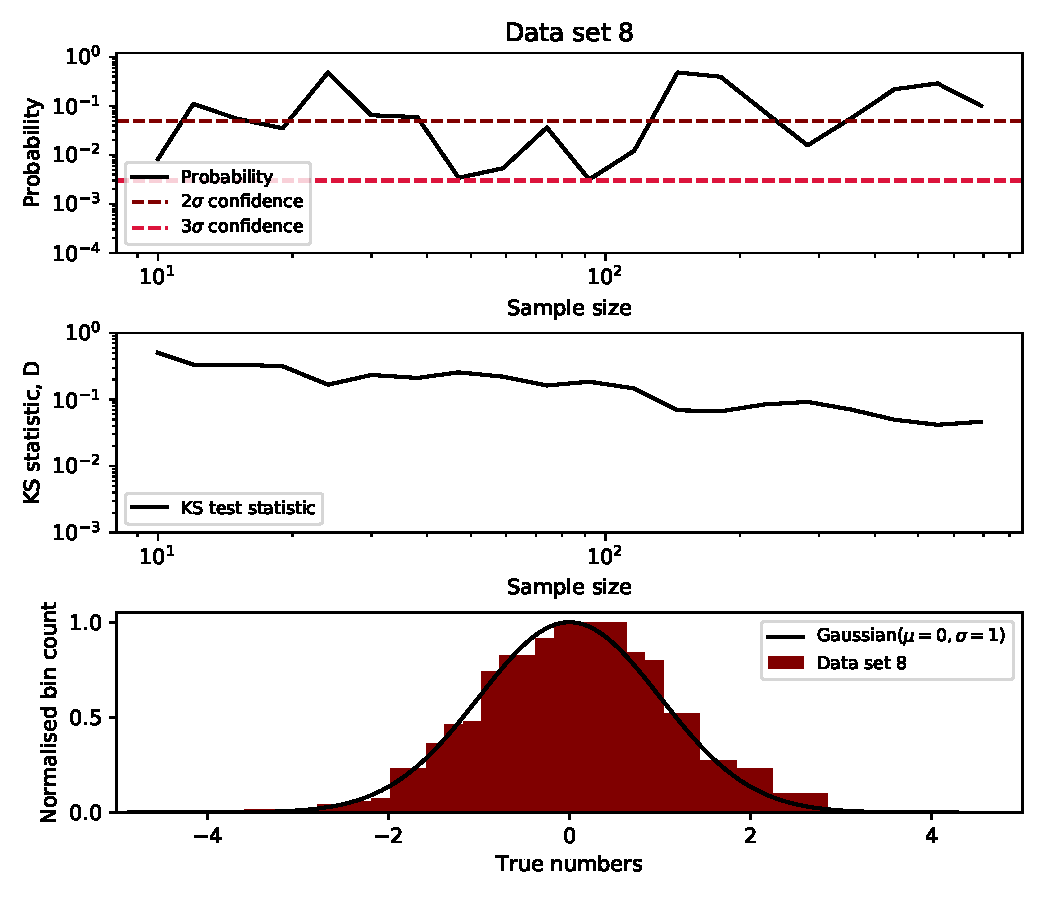
\includegraphics[width = 7.6cm]{./plots/KStest-set8.pdf}
    \caption{\textbf{Upper}: Probability that set 8 matches with a random normal sample; \textbf{middle}: KS-test statistic value; \textbf{lower}: histogram of data set with overlaid Gaussian.}
    \label{fig:KS-8}
\end{minipage}%
\end{figure}

\begin{figure}[!h]
\centering
\begin{minipage}[t]{7.6cm}
    \centering
    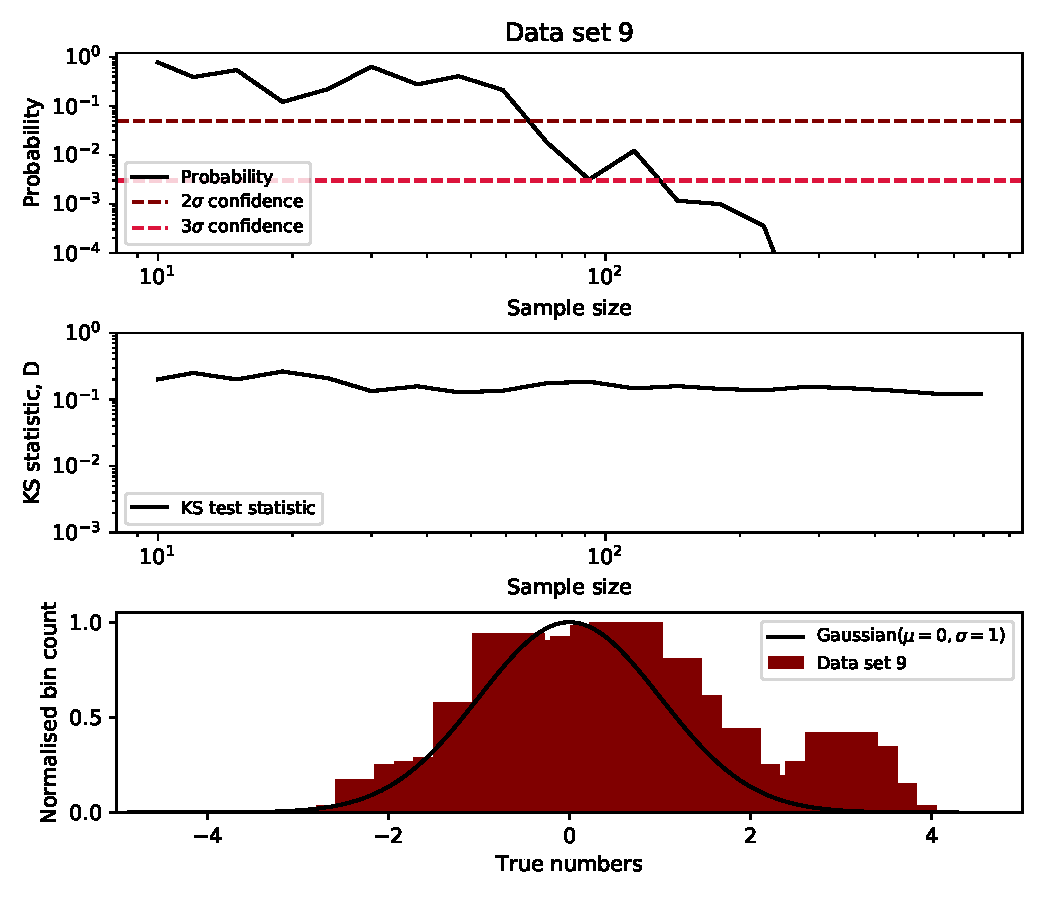
\includegraphics[width = 7.6cm]{./plots/KStest-set9.pdf}
    \caption{\textbf{Upper}: Probability that set 9 matches with a random normal sample; \textbf{middle}: KS-test statistic value; \textbf{lower}: histogram of data set with overlaid Gaussian.}
    \label{fig:KS-9}
\end{minipage}%
\qquad
\begin{minipage}[t]{7.6cm}
    \centering
    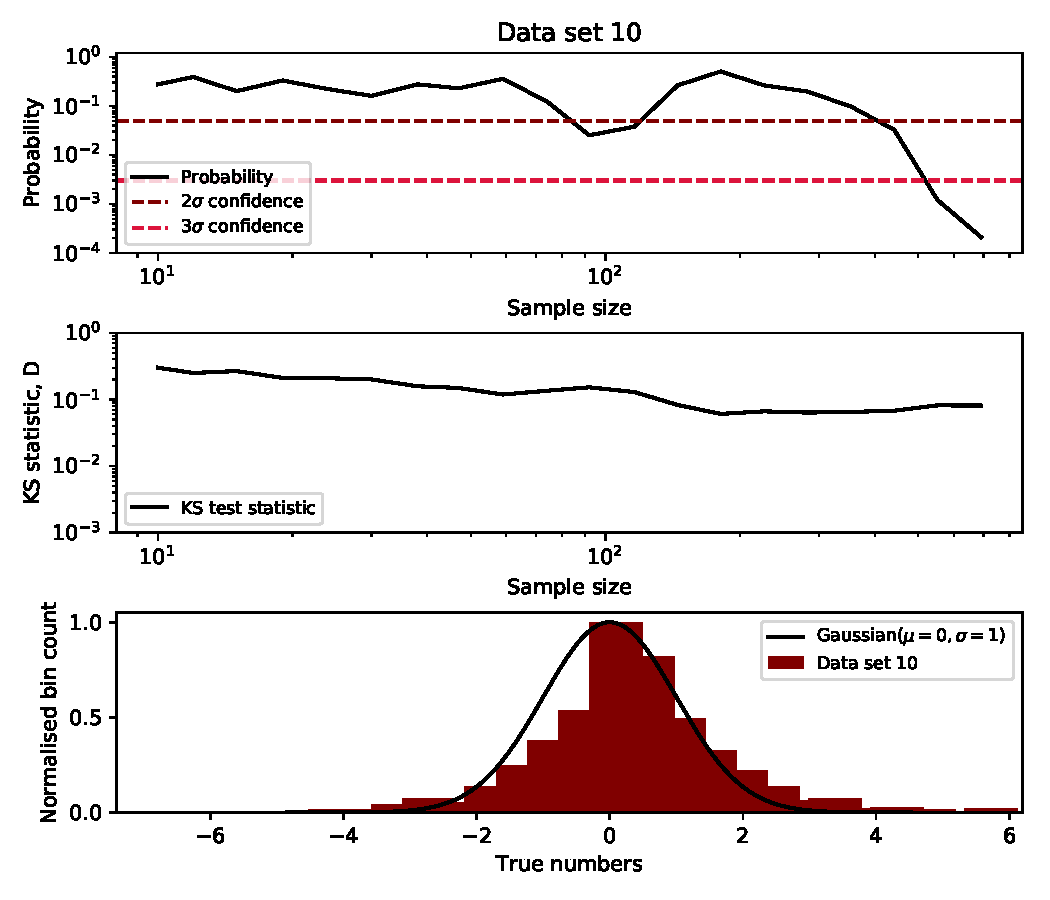
\includegraphics[width = 7.6cm]{./plots/KStest-set10.pdf}
    \caption{\textbf{Upper}: Probability that set 10 matches with a random normal sample; \textbf{middle}: KS-test statistic value; \textbf{lower}: histogram of data set with overlaid Gaussian. }
    \label{fig:KS-10}
\end{minipage}%
\end{figure}


\section{Exercise 2: Making an initial density field}
For this exercise, a Fourier plane is generated. This is done by first creating a random 2D field where the entries are just numbers drawn from a standard normal distribution, and are then Fourier transformed. An amplitude is calculated for each point in the grid, such that it obeys the power spectrum functional form, i.e. the numbers are multiplied by $\sigma$ (equivalent to the mapping function) so that they are now drawn from $G(\mu=0, \sigma)$, where $\sigma^2 = P(k) = k^n$. Here $k^2 = k_x^2+k_y^2$, and $k_x$ and $k_y$ are the coordinates of a point in Fourier space. Their indexing is chosen such that the symmetry $\widetilde{Y}(\mathbf{-k}) = \widetilde{Y}^*(\mathbf{k})$ is satisfied. The following code is used to implement and produce three Gaussian random fields with $n$ = -1, -2 and -3:
\lstinputlisting[language=Python, firstline=86]{ex2.py}

The code output shows the seed, some statistics on the field, and the time elapsed:
\lstinputlisting{./output/ex2.txt}

As seen from the code output, after the inverse Fourier Transform the imaginary parts of the complex numbers are just a very small fraction of $\sim 10^{-10}$ of the real parts, so for the plotting are taken the absolute values, but the imaginary parts have virtually no contribution to this. We can say that the symmetry condition is then fulfilled. In fact, the imaginary parts will hardly be zero as there is always the machine error when the FT and IFT are done (using \verb+numpy+ in this part), so these values seem sensible for a random Gaussian field.

The code has produced plots of the 3 Gaussian random fields, figures \ref{fig:G1}, \ref{fig:G2} and \ref{fig:G3}. The physical size given in these plots is (rather arbitrarily) in $kpc$. This means, in Fourier space, the k vectors are in $kpc^{-1}$. Using different numbers of $n$ obviously impacts the structure formed in the Fourier grid: for $n=-1$, all structures are on very small scales of individual pixels (i.e. 1-2 kpc), and the maximum $k$ amplitude is around 0.025, whereas for $n=-2$, the maximum amplitude is lower, around 0.008, the minimum $k$ is also lower, and structure has formed on larger scales, around $10^2$ kpc. `Clouds' of overdensities have now formed. With $n=-3$, the sctructures look more `collapsed' even, and are on scales of hundreds of kpc, with the underdense region bounds looking more prominent (less `cloudy'). The maximum and minimum amplitudes are lower again, compared to higher $n$ values.

\begin{figure}[!h]
\centering
\begin{minipage}[t]{7.8cm}
    \centering
    \includegraphics[width = 7.8cm]{./plots/GaussianField-1.pdf}
    \caption{Gaussian field with $n = -1$.}
    \label{fig:G1}
\end{minipage}
\qquad
\begin{minipage}[t]{7.8cm}
    \centering
    \includegraphics[width = 7.8cm]{./plots/GaussianField-2.pdf}
    \caption{Gaussian field with $n = -2$}
    \label{fig:G2}
\end{minipage}
\end{figure}

\begin{figure}
    \centering
    \includegraphics[width = 8 cm]{./plots/GaussianField-3.pdf}
    \caption{Gaussian field with $n = -3$}
    \label{fig:G3}
\end{figure}

\section{Exercise 3: Linear structure growth}
In this exercise we solve a 2nd order linear ordinary differential equation (ODE), given by
\begin{equation}
    \frac{d^2 D}{dt^2}+2\frac{\dot{a}}{a}\frac{dD}{dt} = \frac{3}{2}\Omega_0 H_0^2\frac{1}{a^3}D \ .
\end{equation}
We look at an Einstein-de Sitter Universe with purely matter, i.e. $\Omega_m=1$, where the scale factor $a$ is given by
\begin{equation}
    a(t) = \left(\frac{3}{2}H_0 t\right)^{2/3} \ .
\end{equation}
Simplifying (2) using $a$ from (3), we arrive at the equation
\begin{equation}
    \frac{d^2 D}{dt^2} + \frac{4}{3t}\frac{dD}{dt} = \frac{2}{3}\frac{D}{t^2} \ , 
\end{equation}
which has a solution 
\begin{equation}
    D(t) = c_1 t^{2/3} + \frac{c_2}{t} \ .
\end{equation}
In the question we are asked to solve it using the following boundary conditions, which then solve for the constants $c_1$ and $c_2$:
\begin{itemize}
    \item Case 1: $D(1) = 3$, $D`(1) = 2 \quad => \quad$ solution $D(t) = 3t^{2/3}$ 
    \item Case 1: $D(1) = 10$, $D`(1) = -10 \quad => \quad$ solution $D(t) = \frac{10}{t}$ 
    \item Case 1: $D(1) = 5$, $D`(1) = 0 \quad => \quad$ solution $D(t) = 3t^{2/3} + \frac{2}{t}$ 
\end{itemize}

The ODE is solved for these 3 cases numerically using the Runge-Kutta 5th order method, for $t = 1$ yr until $t = 1000$ yr. The code implementation for the method and solving the equation is given by:
\lstinputlisting[language=Python]{ex3.py}

The code output is just the seed values, and the code has also produced 3 plots.
\lstinputlisting{./output/ex2.txt}

The plots are shown on figures  \ref{fig:D1} to \ref{fig:D3}. As seen from the plots, for all 2 cases of initial conditions, the numerical solution (black line) overlaps with the analytical solution, shown in a blue dotted line. A 5th order Runge-Kutta was implemented for this exercise, however using it does little effect compared to the RK4 one, both in terms of accuracy or speed, as this particular coupled ODE system is not numerically hard to solve.
\begin{figure}[!h]
\centering
\begin{minipage}[t]{7.8cm}
    \centering
    \includegraphics[width = 7.8cm]{./plots/growth-factor-1.pdf}
    \caption{Density growth factor for initial conditions case 1 solved with a RK5 algorithm (black full line), compared to the analytical solution (blue dotted line).}
    \label{fig:D1}
\end{minipage}
\qquad
\begin{minipage}[t]{7.8cm}
    \centering
    \includegraphics[width = 7.8cm]{./plots/growth-factor-2.pdf}
    \caption{Density growth factor for initial conditions case 2 solved with a RK5 algorithm (black full line), compared to the analytical solution (blue dotted line).}
    \label{fig:D2}
\end{minipage}
\end{figure}
\begin{figure}[!h]
    \centering
    \includegraphics[width=8cm]{./plots/growth-factor-3.pdf}
    \caption{Density growth factor for initial conditions case 3 solved with a RK5 algorithm (black full line), compared to the analytical solution (blue dotted line).}
    \label{fig:D3}
\end{figure}

\section{Exercise 4: Zeldovich approximation}

\subsection{Part a: calculating the linear growth factor for redshift z=50}
The linear growth factor is given by the expression
\begin{equation}
    D(z) = \frac{5\Omega_m H_0^2}{2}H(z)\int_z^\infty{\frac{1+z'}{H^3(z')}dz'} \ ,
\end{equation}
where $z$ is redshift, $\Omega_m = 0.3$ is the matter fraction of the Universe at $z = 0$, $H_0$ 0 is the Hubble constant at $z = 0$, and $H(z)$ is given by
\begin{equation}
    H(z) = H_0\sqrt{\Omega_m(1+z)^3+\Omega_{\Lambda}} \ ,
\end{equation}
where $\Omega_{\Lambda} = 0.7$ is the e dark energy fraction of the Universe. To calculate the growth factor at $z = 50$ we can use numerical integration to solve equation (6) and find the value of the integral. If the expression is given in terms of $z$, the upper bound of the integral is infinity, which is not particularly desirable. Although we can, in principle, integrate to a high enough value of $z$ e.g. 1000 and claim the result should converge, it is more useful to use the substitution $a = 1/(z+1)$. Hence, substituting, using $z = 1/a - 1$ and then $dz/da = -1/a^2$, changing the limits of the integral from $z$ to $a$ and $\infty$ to $0$ and swapping them to absorb the minus sign in $da$, expression (6) becomes:
\begin{equation}
    D(a) = \frac{5\Omega_m H_0^2}{2}H(a)\int_0^{a} \frac{1/a^3}{H_0^3(\Omega_m/a^3 + \Omega_{\Lambda})^{3/2}}da \ ,
\end{equation}
and here $H(a)$ can be calculated using just $H(1/(1+z))$. Expression (8) can be simplified further if $H(a)$ is substituted into the equation, to lead to
\begin{equation}
    D(a) = \frac{5\Omega_m}{2}\left(\frac{\Omega_m}{a^3}+\Omega_{\Lambda}\right)^{1/2 }\int_0^{a} \frac{1/a^3}{(\Omega_m/a^3 + \Omega_{\Lambda})^{3/2}}da \ .
\end{equation}
Note that the Hubble constant $H_0$ has simplified in the equation. The following code is used to
\begin{itemize}
    \item Numerically calculate the integral in expression (9), implemented in function \verb+growth_factor_a()+, with the numerical integration routine in the function \verb+integrate()+, with an accuracy of 1e-10, from $a = 0 \ (z = \infty)$ to $a = 1/51 \ (z = 50)$. The result is saved in the variable \verb+A+.
    \item Calculate the linear growth factor $D(a=1/51)$ using the simplified version of (6), equation (10), saved in the variable \verb+D+. 
    \item Print \verb+A+ and \verb+D+ in the output.
\end{itemize}
\lstinputlisting[language=Python]{ex4a.py}

The code output is given by:
\lstinputlisting{./output/ex4a.txt}

The value for the integral obtained through the numerical integration routine matches to the 6th figure the value given by Wolfram Alpha. Also, the value of the growth factor is in agreement with values given by cosmological calculators, which for the given parameters give $D(z=50) \approx 0.0196$.

\subsection{Part b: calculating the derivative of the linear growth factor}
The derivative of the linear growth factor, obtained indirectly, is given by
\begin{equation}
    \dfrac{dD(t)}{dt} = \frac{dD}{da}\dot{a}\ , 
\end{equation}
given that we know $\dot{a} = H(z)a(z)$. Differentiating (9) with respect to $a$ and substituting $\dot{a}$ gives:
\begin{equation}
    \dot{D} = \frac{5\Omega_m}{2}\frac{1}{2}\left(-3\frac{\Omega_m}{a^4} \right)\left(\frac{\Omega_m}{a^3}+\Omega_{\Lambda}\right)^{-1/2} a H_0 \left(\frac{\Omega_m}{a^3} + \Omega_{\Lambda}\right)^{1/2} \int_0^{a} \frac{1/a^3}{(\Omega_m/a^3 + \Omega_{\Lambda})^{3/2}}da \ ,
\end{equation}
where we notice that the 3rd term in the brackets simplifies with the 5th term (both taken from $H(a)$). Simplifying further, we reach
\begin{equation}
    \dot{D} = -\frac{15}{4}\Omega_m^2 H_0 \frac{A}{a^3} \ , 
\end{equation}
where $A$ is the numerical value of the integral calculated in part 4a. Substituting for it, $\Omega_m$, $H_0$ and $a = 1/51$, we get the answer:
\begin{equation}
    \boxed{\dot{D}|_{a = 1/51} = -4.20092365\times10^{-10}} \ .
\end{equation}

The following code calculates this number by calculating the value of $A$ as in 4a, and plugging the numbers in equation (12). It also calculates the derivative numerically, where the function being differentiated is given in the \verb+D_a()+ function, and the algorithm implemented for numerical differentiation is in \verb+differentiate_at_point()+. It then outputs both numbers.
\lstinputlisting[language=Python, firstline=34]{ex4b.py}

The code output is:
\lstinputlisting{./output/ex4b.txt}

As seen from the code output, the numerical and analytical derivative values match up to the 8th significant figure and further. The value is so small because of the multiplication with the Hubble constant in the given units, 1/years, which is of the order of $10^{-11}$.

\section{Exercise 5: Mass assignment schemes}
\subsection{Part a: Implementing the nearest grid point method}
The nearest grid point method is called like this because, given a grid divided in cells, when a point is put in the grid, we assign all of its mass to the grid point that is nearest (in coordinates) to the point we have just put. This way, all the mass we `put' in the grid is there, except assigned to a point with coordinates that belong to the grid points exactly, and not somewhere inbetween. The following code does some supplementary things:
\begin{itemize}
    \item Creates a cubic grid with side 16 of class \verb+Grid+. Upon declaration, the \verb+init+ method initialises the cells of the grid such that it now contains cells of class \verb+Cell+ that have an index and boundaries in 3 dimensions, as well as width. Also, grid points are initialised, such that they have 3 indices and are now more easily traceable/plottable. 
    \item The \verb+assign_masses_ngp()+ function assigns masses to the grid points using the Nearest Grid Point mass assignment scheme. The arguments passed to the function are the positions of the particles inserted in the 3D grid, their masses are, for now, assumed to be unity, although this can easily be generalised, but as this method doesn't require it the function only adds a value of one to the cell the particle belongs to. A cell by itself is defined by only one grid point (its boundary coordinates $x, y, z$ and its width are enough). Hence, assigning the mass to a cell is equivalent to assigning it to the point of the grid that corresponds to this cell uniquely.
    \item For plotting $x-y$ slices at $z$ values of 4, 9, 11 and 14, the code finds the grid points in this plane and adds them to a plot. Also, the newly added points whose $z$ values are within a tolerance of 0.05 of the aforementioned slices are plotted with red points. Obviously, when 1024 are randomly put in a $16^3$ grid, we don't expect any of them to lie exactly in the slice with integer $z$, so this tolerance is applied.
    \item The plots produced by the following script are shown on figures \ref{fig:s4} to \ref{fig:s14}.
\end{itemize}

\lstinputlisting[language=Python]{ex5a_supplementary.py}

\begin{figure}[!h]
\centering
\begin{minipage}[t]{7.8cm}
    \centering
    \includegraphics[width = 7.8cm]{./plots/grid-slice-4.pdf}
    \caption{Slice of grid at z = 4 and points that fall in this plane with a tolerance of 0.05 shown in red.}
    \label{fig:s4}
\end{minipage}
\qquad
\begin{minipage}[t]{7.8cm}
    \centering
    \includegraphics[width = 7.8cm]{./plots/grid-slice-9.pdf}
    \caption{Slice of grid at z = 9 and points that fall in this plane with a tolerance of 0.05 shown in red.}
    \label{fig:s9}
\end{minipage}
\end{figure}

\begin{figure}[!h]
\centering
\begin{minipage}[t]{7.8cm}
    \centering
    \includegraphics[width = 7.8cm]{./plots/grid-slice-11.pdf}
    \caption{Slice of grid at z = 11 and points that fall in this plane with a tolerance of 0.05 shown in red.}
    \label{fig:s11}
\end{minipage}
\qquad
\begin{minipage}[t]{7.8cm}
    \centering
    \includegraphics[width = 7.8cm]{./plots/grid-slice-14.pdf}
    \caption{Slice of grid at z = 14 and points that fall in this plane with a tolerance of 0.05 shown in red.}
    \label{fig:s14}
\end{minipage}
\end{figure}

The following code produces plots of the values of the cells when the masses are assigned to the grid points using a colour plot and \verb+imshow+:
\lstinputlisting[language=Python]{ex5a.py}

The figures produced are the four slices, shown on figures \ref{fig:slice4} to \ref{fig:slice14}.

\begin{figure}[!h]
\centering
\begin{minipage}[t]{7.8cm}
    \centering
    \includegraphics[width = 7.8cm]{./plots/slice-4.pdf}
    \caption{Slice of grid at z = 4 and colourbar representing the mass value of the corresponding cell.}
    \label{fig:slice4}
\end{minipage}
\qquad
\begin{minipage}[t]{7.8cm}
    \centering
    \includegraphics[width = 7.8cm]{./plots/slice-9.pdf}
    \caption{Slice of grid at z = 9 and colourbar representing the mass value of the corresponding cell.}
    \label{fig:slice9}
\end{minipage}
\end{figure}

\begin{figure}[!h]
\centering
\begin{minipage}[t]{7.8cm}
    \centering
    \includegraphics[width = 7.8cm]{./plots/slice-11.pdf}
    \caption{Slice of grid at z = 11 and colourbar representing the mass value of the corresponding cell.}
    \label{fig:slice11}
\end{minipage}
\qquad
\begin{minipage}[t]{7.8cm}
    \centering
    \includegraphics[width = 7.8cm]{./plots/slice-14.pdf}
    \caption{Slice of grid at z = 14 and colourbar representing the mass value of the corresponding cell.}
    \label{fig:slice14}
\end{minipage}
\end{figure}

\subsection{Part b: Individual cells}
The following code uses the function \verb+get_value()+ to calculate the value that would be assigned to cell 4 or cell 0 if a particle is found in the domain of all possible positions in $x$:
\lstinputlisting[language=Python]{ex5b.py}

The code has produced figures \ref{fig:pass4} and \ref{fig:pass0}, which look like a top-hat function where the function would assign a value to the given cells.

\begin{figure}
    \centering
    \includegraphics[width=11cm]{./plots/passing-particle-4.pdf}
    \caption{Value of cell 4 when a particle `passes' through the grid domain in x.}
    \label{fig:pass4}
\end{figure}

\begin{figure}
    \centering
    \includegraphics[width=11cm]{./plots/passing-particle-0.pdf}
    \caption{Value of cell 0 when a particle `passes' through the grid domain in x.}
    \label{fig:pass0}
\end{figure}

\section{Exercise 6: Classifying gamma-ray bursts}

\section{Exercise 7: Building a Barnes-Hut quadtree}
In this exercise we implement a Barnes-Hut quadtree,  where the particles are taken from the file \verb+colliding.hdf5+. The problem here is two-dimensional, with only the $x$ and $y$ coordinates of the particles being considered. The code does the following:
\begin{itemize}
    \item Reads data for the particles and creates \verb+gals+ of class \verb+QuadTree+ with width and height of 150, starting at (0, 0). 
    \item Adds points to the tree (of the \verb+Point+ class) using \verb+gals.add_point+, where the coordinate, the mass and ID of each particle is given.
    \item \verb+gals.subdivide()+ recursively divides the tree into nodes until each node has no more than the \verb+point_limit+ = 12 particles.
    \item Visualises the quadtree with \verb+gals.graph()+ which plots all points and the nodes they belong to in rectangle patches. It also plots a zoom-in region that shows the two galaxies more closely.
    \item \verb+gals.calculate_multipole()+ calculates the $n=0$ multipole moment of each leaf and node of the tree, which is just the sum of the masses of all particles in the given node, $M_0 = \scriptscriptstyle\displaystyle\sum_{a\ in\ node}m_a$ . 
    \item Recursively searches for the point with index $i = 100$ with the function \verb+search_point()+, which additionally outputs the $n=0$ multipole moment for each node containing this particle including the root, and the coordinates of the node's cell. For confirmation, the true coordinates of the point are also printed out, and a plot of the quadtree is made again, in which the point of search is indicated with a blue cross. 
\end{itemize}
\lstinputlisting[language=Python]{ex7.py}

The code also contains a commented out section with a test putting 100 random particles in a tree and subdividing it until each point is alone in its node. The code output is:
\lstinputlisting{./output/ex7.txt}

The tree plots produced of the visualisation of the tree are figures \ref{fig:Quadtree}, \ref{fig:Quadtree-zoom}, and \ref{fig:Quadtree-point}.

\begin{figure}[!h]
\centering
\begin{minipage}[t]{7.8cm}
    \centering
    \includegraphics[width = 7.8cm]{./plots/quadtree.pdf}
    \caption{Visualisation of quadtree of two colliding galaxies.}
    \label{fig:Quadtree}
\end{minipage}
\qquad
\begin{minipage}[t]{7.8cm}
    \centering
    \includegraphics[width = 7.8cm]{./plots/quadtree-zoom.pdf}
    \caption{Zoom around the two galaxies in the quadtree.}
    \label{fig:Quadtree-zoom}
\end{minipage}
\end{figure}

\begin{figure}
    \centering
    \includegraphics[width = 8.5cm]{./plots/quadtree-point.pdf}
    \caption{Visualisation of quadtree with the point with index i = 100 marked with a blue cross. The nodes that contain it are printed (with their box coordinates and n = 0 multipole moments) in the output of the ex7.py script.}
    \label{fig:Quadtree-point}
\end{figure}

\end{document}
